% Chapter 3

\chapter{Solution n° 2} % Main chapter title

\label{Chapter3} % For referencing the chapter elsewhere, use \ref{Chapter3} 

%----------------------------------------------------------------------------------------

Nous avons trouvé un driver imx219.c compatible avec une version 3.14 du kernel soit
version Jethro de Yocto. Disponible à cette adresse : \\ \\
\href{https://chromium.googlesource.com/chromiumos/third_party/kernel/+/factory-ryu-6486.14.B-chromeos-3.14/drivers/media/i2c/soc_camera/imx219.c}{https://chromium.googlesource.com/chromiumos/third\_party/kernel/+/factory-ryu-6486.14.B-chromeos-3.14/drivers/media/i2c/soc\_camera/imx219.c} \\

Le driver imx219 contient toutes les fonctions permettant la configuration de l’imx219
(on, off, gain, couleurs., taille de l’affichage..) via le driver i2c et le driver v4l.
Lors du chargement du module, l’imx219 est automatiquement configuré par v4l. Cette
configuration permet de modifier certains paramètres du flux vidéo à l’aide des fonctions
contenues dans le driver imx219. Le flux peut être ensuite récupéré avec les commandes de
Gstreamer ou de v4l-utils.

Gstreamer permettrait de streamer le flux sur le réseau à travers le protocole UDP alors
que v4l-utils permettrait plutôt d’enregistrer le flux vidéo.

Nous avons commencé par compiler le driver sans l’intégrer directement au système
(linux-openrex) par l’utilisation de patchs mais en réalisant une recette qui compilera
le fichier.

\begin{figure}[th]
    \centering
    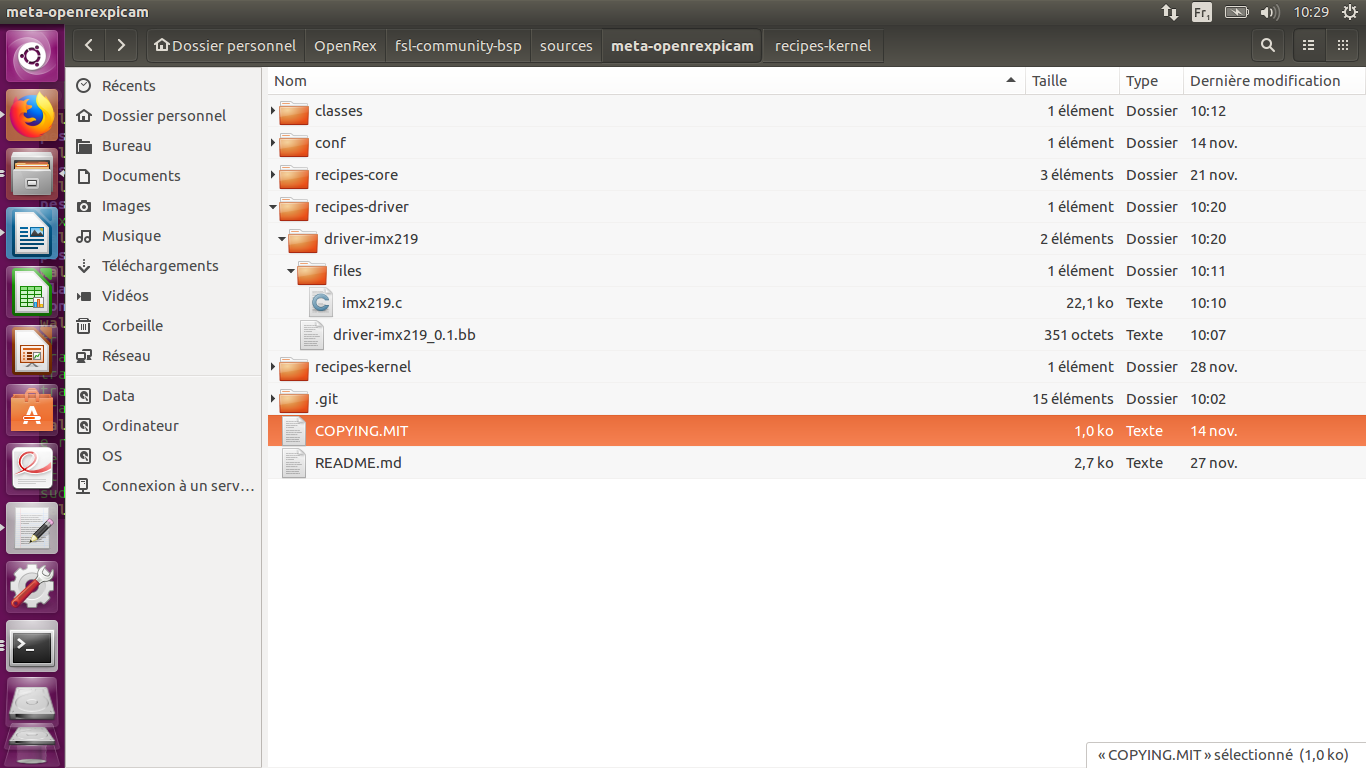
\includegraphics[width=1\linewidth,trim={9,5cm 14,5cm 15cm 6,7cm},clip]{arborescence.png}
    \decoRule
    \caption{Arborescnce des fichiers}  \label{fig:arbor}   
\end{figure}

Extrait de la recette : Elle permet de récupérer le fichier imx219.c de le compiler par la cross tool-chain et de l’installer.

\begin{figure}[th]
    \centering
    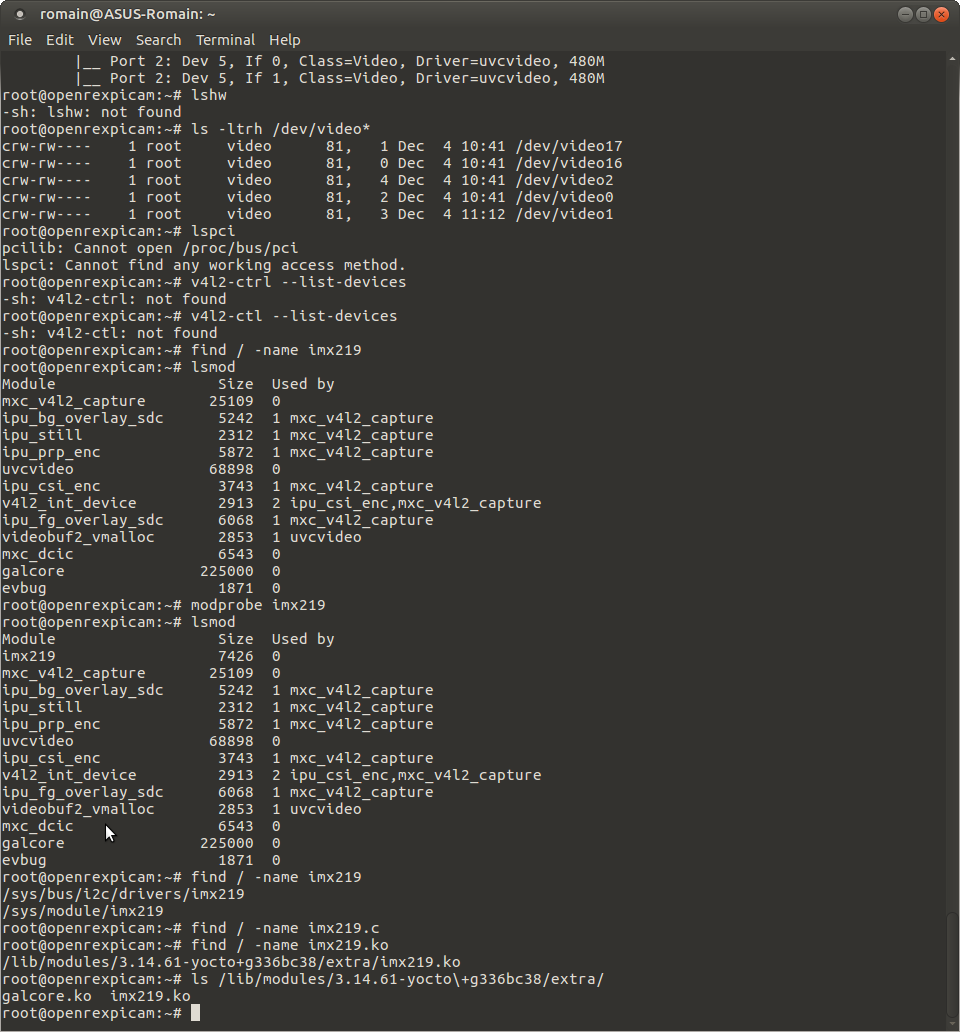
\includegraphics[width=1\linewidth,trim={0cm 1cm 0cm 33,1cm},clip]{presence.png}
    \decoRule
    \caption{Vérification de la présence du driver}  \label{fig:pres}   
\end{figure}

\clearpage

\begin{lstlisting}
SUMMARY = "driver imx219"
SECTION = "examples"
LICENSE = "MIT"
LIC_FILES_CHKSUM = "file://${COMMON_LICENSE_DIR}/MIT;md5=c2b5f7071fdde268bf46ace1546f3c4b"
    
SRC_URI = "file://imx219.c"
S = "${WORKDIR}"
    
do_compile() {
    ${CC} imx219.c -o imx219
}
    
do_install() {
    install -d ${D}${bindir}
    install -m 0755 imx219 ${D}${bindir}
}
\end{lstlisting}

Chargement du module imx219 :

\begin{figure}[th]
    \centering
    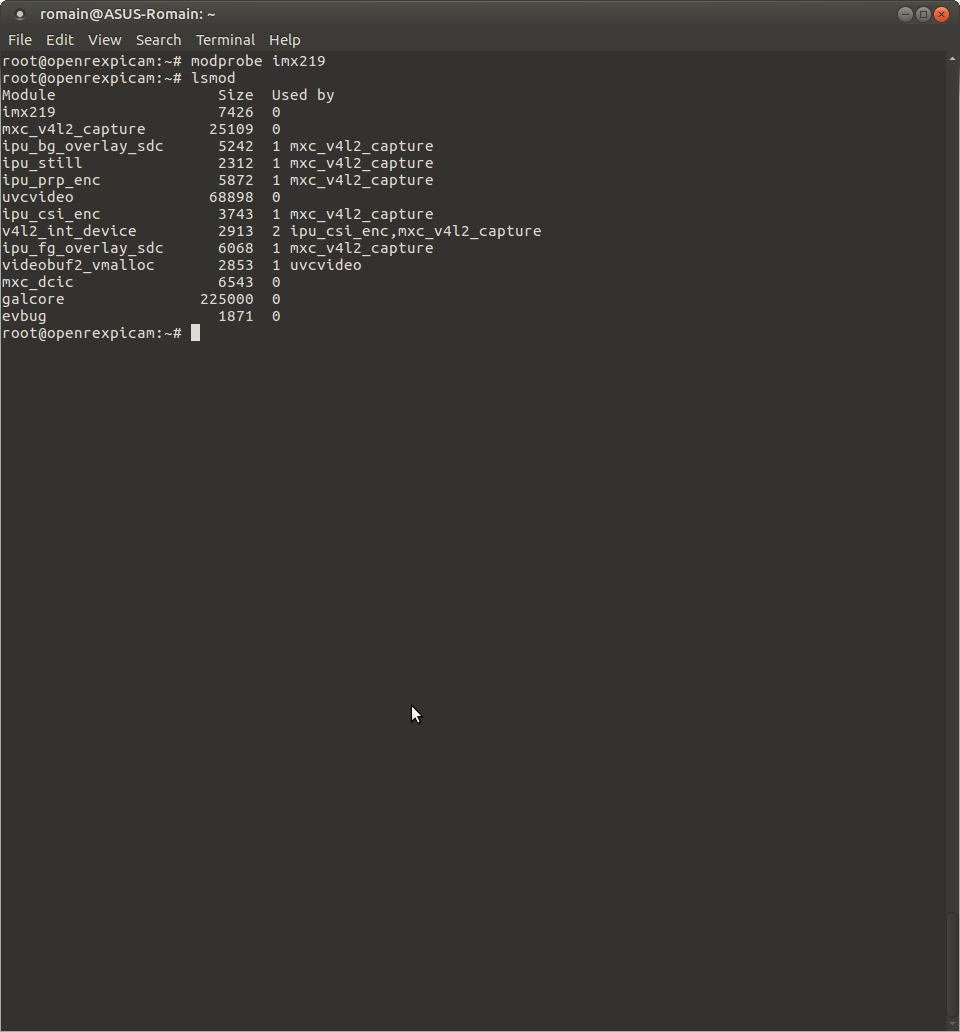
\includegraphics[width=1\linewidth,trim={0cm 25cm 0cm 1,8cm},clip]{module.png}
    \decoRule
    \caption{Chargement du module}  \label{fig:mod}   
\end{figure}

Comme nous pouvons le voir le driver n’est pas encore utilisé par v4l (Used by 0).
Chargement du module à l’adresse I2C de l’imx219 :

\begin{figure}[th]
    \centering
    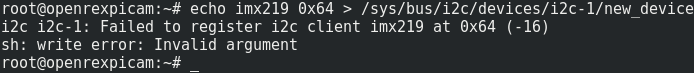
\includegraphics[width=1\linewidth]{modadd.png}
    \decoRule
    \caption{Chargement du module avec l'adresse I2C}  \label{fig:modadd}   
\end{figure}

Nous arrivons à une erreur sur le bus i2c sur laquelle nous travaillons actuellement.
Récupération du flux vidéo en local via Gstreamer :

\textbf{\# gst-launch-1.0 v4l2src device="/dev/videoX" ! video/x-raw,width=640,height=480 ! autovideosink}

X’ étant le numéro correspondant au numéro du driver vidéo du port CSI-2

Nous sommes actuellement entrain de chercher des pistes sur l’utilisation des commandes
gst-launch-1.0 et les fichiers de configurations v4l2src la suite de cette partie sera
développer à la suite de ce rapport. 

%----------------------------------------------------------------------------------------